\documentclass{report}
\usepackage{tabularx}
\usepackage{listings}
\usepackage{graphicx}
\usepackage{fixlatvian}
\usepackage{tikz}
\usepackage{circuitikz}
\usepackage{pgfplots}

\title{"Vienkāršu elektrisku shēmu modelēšana"}
\author{Dmitrijs Koršunovs REBM01}
\date{April 2018}

\begin{document}

\maketitle
\chapter{Teorētiskā dalļa}
\section{Ķēdes aprēķins}
Šajā uzdevumā studentiem bija uzdots aprēķināt spriegumu uz diviem rezistoriem virknes sleguma ķēdē, kurā izņemot rezistorus, ir vel līdzsprieguma avots. Spriegums āvotam ir mana studenta apliecības pēdēji trīs cipari, dalīti ar 10 vērtība, tas ir 19,9V. Rezistoru pretestības lielumi ir apliecības pēdējas 3 ciparu otrais numurs+1, bet otrā rezistora vērtība ir numura pēdējais cipars+1, manā gadījumā bus $R_1=10\Omega$ un $R_2=10\Omega$.
Pēc manu datu ievietošanu sprieguma dalītāja formulā:\\
\begin{figure}[!h]
\centering
\noindent$U_1 = \frac{R_1}{R_1 + R_2}*U_1 =\frac{10}{10 + 10}*19.9 = 9.95 V $\\\ $U_1 = \frac{R_2}{R_1 + R_2}*U_1 =\frac{10}{10 + 10}*19.9 = 9.95 V $\\
\caption{Aprēķinu formulas}
\end{figure}
\label{Darba_tabula}
\par
\begin{table}[!h]
\centering
\begin{tabular}{|c|c|}
\hline
     $R_1$&$10\Omega$ \\
\hline
     $R_2$&$10\Omega$\\
\hline
     $V_1$&$19.9V$ \\
\hline
     $U_R1$&$9.95V$\\
\hline
     $U_R2$&$9.95V$\\   
\hline

\end{tabular}
\caption{Darba tabula}
\end{table}
\chapter{Praktiskā daļa}
\subsection{Darbs ar GEDA programmām}
\subsection{darbs ar gshem}
\begin{figure}[!h]
\includegraphics[width=12cm]{01_sch.png}
\caption{mana varianta dotā shēma}
\end{figure}
\subsection{darbs ar gnetlist}
\lstinputlisting{01.net}
\subsection{Darbs ar ngspice}
\begin{figure}[!h]
\includegraphics[width=12cm]{results.png}
\includegraphics[width=6.5cm]{01.png}
\includegraphics[width=6.5cm]{01.png}
\caption{Simulācijas sprieguma rezultāti 2 mezglos un 2 rezistoru voltampēra raksturliknes}
\end{figure}
\section{Darbs ar QUCS programmām}
\begin{figure}[!h]
\centering
\includegraphics[width=12cm]{qucs_circuit.png}
\caption{Šeit ir redzama principiālā shēma, kas bija sastadīta pēc uzdevuma dotiem datiem}
\end{figure}
\label{rer}

\begin{figure}[!h]
\centering
\includegraphics[width=9cm]{DC.png}
\caption{Te mēs redzam strāvas atkarību no 2.rezistora lieluma izmaiņas}
\end{figure}

\begin{figure}[!h]
\centering
\includegraphics[width=9cm]{Voltage.png}
\caption{Sweep simulācijas grafiks}
\end{figure}

\begin{figure}[!h]
\centering
\includegraphics[width=9cm]{table.png}
\caption{Sweep simulācijas tabula}
\end{figure}

\begin{figure}[h!]
\begin{center}
\begin{circuitikz}[american]
\draw (0,2) to[V=$U_s$] (0,0);
\draw (3,2) to[R=$R_1$] (3,0);
\draw (2,2) to[R=$R_2$] (1,2);
\draw (0,2) to[short] (1,2);
\draw (2,2) to[short] (3,2);
\draw (3,0) to[short] (0,0);
\end{circuitikz}
\caption{Mana shēma}
\end{center}
\end{figure}

\begin{figure}[h!] 
\begin{center}
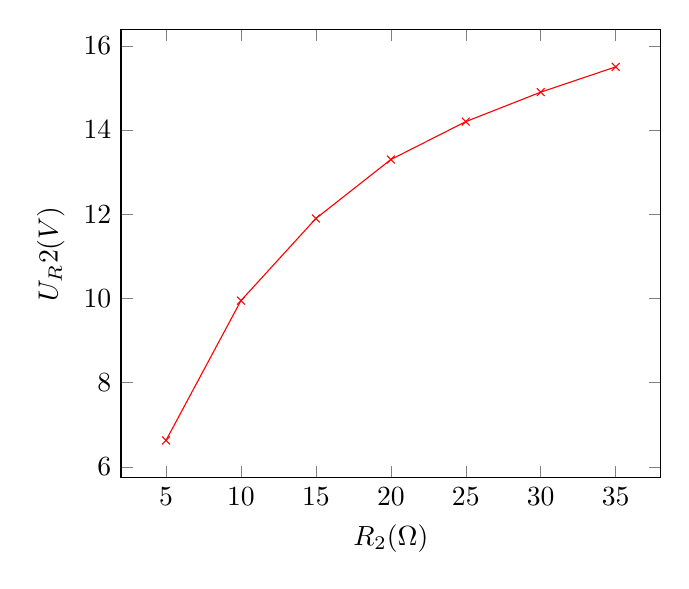
\begin{tikzpicture}
	\begin{axis}[
		xlabel=$R_2 (\Omega)$,
		ylabel=$U_R2 (V)$]
	\addplot[color=red,mark=x] coordinates {
		(5,6.63)
		(10,9.95)
		(15,11.9)
		(20,13.3)
		(25,14.2)
		(30,14.9)
		(35,15.5)
	};
	\end{axis}
\end{tikzpicture}
\caption{shēmas UR2 = f(R2) grafiks}
\label{fig:graf}
\end{center}
\end{figure}


\chapter{Atsauksmes}
Beigās gribētu minēt dažas vietnes. \cite{plots} mājaslapi no literatūras saraksta, kur es paņēmu paraugu sastādot \ref{fig:graf} grafiku, un \cite{bibly} mājaslapu no literatūras saraksta, kur es paskatījos, kā pareizi sastadīt literatūras sarakstu dokumenta beigās.


\begin{thebibliography}{9}
\bibitem{plots}\texttt{http://pgfplots.sourceforge.net/gallery.html}

\bibitem{bibly}\texttt{https://www.sharelatex.com/learn/Bibliography\\\textbackslash\_management\textbackslash\_with\textbackslash\_bibtex}

\end{thebibliography}

\end{document}


